\chapter{Detection Performance}

In this chapter we will present the performance for the basline and iVector system both for open and closed set detection.

\section{Baseline System on 30 Second Utterances}

In figure \ref{fig:basedet30} the DET-curve for the baseline system is shown. The system achieved an $C_{\text{Det}}$ of $0.0330$ for the closed set and $0.0478$ for the open set evaluations. From the DET-curve we see that the miss probability cannot be reduced to below about $4$\% without a severe increase in false alarms. This might be because the bayesian models are capable of discriminating classes, even though they give poor probability estimates \cite{mccallum1998comparison}. Usually the score-vector (which was the probability for each class) used in the backend was dominated by one class with a probability close to $1$. This made the score-vector contain almost no information for alternative suggestions to the dominating class, so the backend had to make blind guesses if it were to further reduce the miss probability below a certain point. The EER is seen to be beyond the point where the miss-probability stagnates, and is $4.91$\% and $4.38$\% for the closed and open set respectively.

\begin{figure}[hbt!]
\begin{center}
	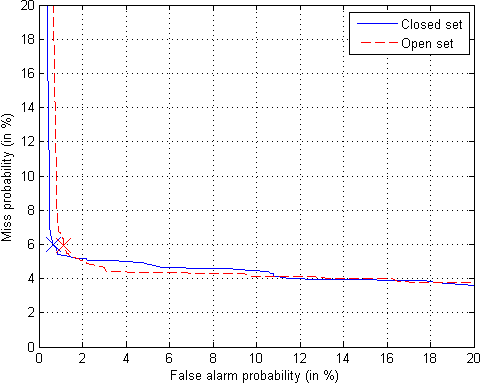
\includegraphics[width=0.8\textwidth]{figures/baseDet30.png}
\end{center}
\caption{Baseline system DET-curves for the 30 second open and closed set NIST utterances. The crosses indicates the miss and false alarm probability used when calculating $C_{\text{Det}}$.}
\label{fig:basedet30}
\end{figure}

%closed c_det 0.032955
%open c_det 0.047809
%closed EER 4.9132
%open EER 4.375

\section{iVector system 30 second performance}

The Det-curves for 30 second utterances recognized by the iVector system is shown in figure \ref{fig:ivectdet30}. A noticeable difference from the baseline system is that this sytem is more adaptable to different requirements for the miss or false alarm probability. Still the $C_{\text{Det}}$ is $0.0353$ and $0.0494$ for the closed and open set respectively which is slightly higher than the baseline system. The EER is however significantly lower, at only $2.76$\% for the closed set and $3.59$\% for the open set. The better EER should probably not be contributed to improved recognition capabilities by iVectors, but rather the shortcomings in the score-vector used by the baseline system. The difference between the open and closed set results suggest like we expected that the assumptions made to incorporate out-of-set languages weren't completely valid. E.g. at the threshold used to calculate $C_{\text{Det}}$, $55$\% of the out-of-set utterances were recognized as target language utterances. 

\begin{figure}[hbt!]
\begin{center}
	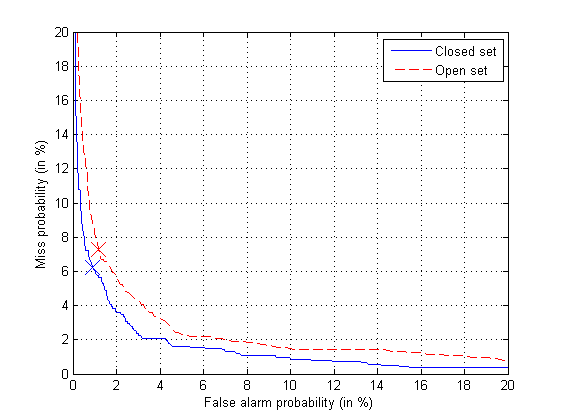
\includegraphics[width=0.8\textwidth]{figures/ivectDet30.png}
\end{center}
\caption{iVector system DET-curves for the 30 second open and closed set NIST utterances. The crosses indicates the miss and false alarm probability used when calculating $C_{\text{Det}}$.}
\label{fig:ivectdet30}
\end{figure}

%closed_cdet 0.035314
%open c_det 0.049353
%closed EER 2.7604
%open  EER 3.5938


\section{Ten and Three Second Performance}

%\begin{table}[hbt!]
%\begin{center}
%\begin{tabular}{| l | c  c | c  c |}
%\cline{2-5}
%\multicolumn{1}{c |}{} & \multicolumn{2}{  c | }{Closed set} & \multicolumn{2}{ c |}{Open set} \\ %\cline{2-5}
%\multicolumn{1}{c |}{} & $C_{\text{Det}}$ & EER (\%) & $C_{\text{Det}}$ & EER (\%) \\
%\hline
%iVector 10 sec. & 0.157 & 13.3 & 0.163 & 13.7 \\
%iVector 3 sec. & 0.259 & 26.5 & 0.264 & 26.8 \\
%\hline
%Baseline 10 sec. & 0.170 & 18.6 & 0.183 & 17.0 \\
%Baseline 3 sec. & 0.351 & 32.0 & 0.437 & 46.8 \\
%\hline
%\end{tabular}
%\end{center}
%\caption{Detection performance for the iVector and baseline system on 3 and 10 second utterances.}
%\label{tab:shortdetrate}
%\end{table}

The DET-curves for the 3 and 10 second tests of the baseline and iVector system are shown in figure \ref{fig:sysdetshort}. The iVector system is seen to outperform the baseline system for these conditions.  There are only minor differences between the open and closed set results, except for the three second baseline performance. This was caused by the backend recognizing more target language utterances than out-of-set utterances as being out-of-set. Although the assumptions made to accommodate shorter utterances in section \ref{sect:ivectshort} seems to fit fairly well, we expect that it is possible to improve these results significantly for both systems. This is supported by the comparison of other systems given in the next section, where the EER for our systems are seen to deterioate faster when the length of the utterances are reduced.

\begin{figure}[hbt!]
	\begin{center}
		\subfloat[ ]{
			\label{fig:ivectdetshort}
			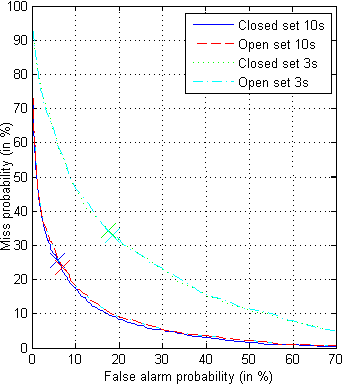
\includegraphics[width=0.42331288343558\textwidth]{figures/ivectDetShort.png}
		}
		\subfloat[ ]{
			\label{fig:basedetshort}
			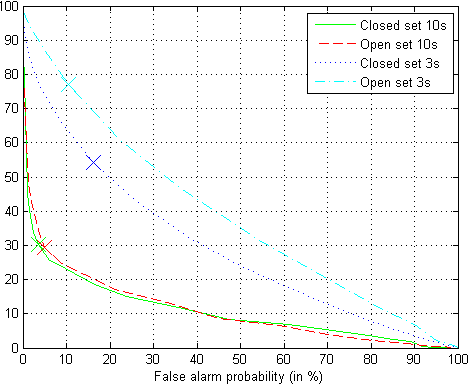
\includegraphics[width=0.57668711656442\textwidth]{figures/baseDetShort.png}
		}
	\end{center}
	\caption{DET-curves of the baseline and iVector system for 10 and 3 second NIST LRE03 utterances. (a) is the iVector performance, (b) is the baseline. The crosses indicates the point where $C_{\text{Det}}$ was calculated from.}
	\label{fig:sysdetshort}
\end{figure}
 
\section{Comparison to Other Systems}

We've listed the performance of the baseline, iVector and 6 other systems in table \ref{tab:compdetresults}. The four systems from MITLL consisted of an trigram PRLM system running in parallell with six phoneme recognizer, an acoustic GMM and SVM VSC system and the fusion of the aforementioned systems. The baseline and iVector system performed competitively against these systems for the 30 second test, but they were surpassed by the fusion system for the shorter durations. 

\begin{table}[hbt!]
\begin{center}
\begin{tabular}{| l | c | c | c | c |}
\hline
System & 30s & 10s & 3s \\
\hline
iVector & 2.8 & 13.3 & 26.5 \\
Baseline & 4.9 & 18.6 & 32.0 \\
\hline
MITLL-PPRLM & 6.6 & 14.3 & 25.5 \\
MITLL-GMM & 4.8 & 9.8 & 19.8 \\
MITLL-SVM & 6.1 & 16.4 & 28.2 \\
MITLL-FUSE & 2.8 & 7.8 & 20.3 \\
\hline
BUT-SPDAT & 2.4 & 8.1 & 19.1 \\
BUT-PRLM &1.8 & 6.6 & 18.8 \\
\hline
\end{tabular}
\end{center}
\caption{EER in \% for an ensamble of language recognition systems for the NIST LRE 2003 closed set evaluations. The MITLL systems are published in \cite{singer2003acoustic}, while the BUT systems are from \cite{matejka2006use}.}
\label{tab:compdetresults}
\end{table}

It is difficult to directly compare the iVector approach to other recognition systems since the performance will heavily depend on the quality of the phoneme transcripts \cite[p. 64]{butphnrec}. The BUT-SPDAT system used four phoneme recognizers for a trigram PPRLM system, but an superior performance was reached by the BUT-PRLM system. The increased recognition capabilities were partially contributed to better phoneme recognition and use of phone lattices \cite{matejka2006use}. The pphoneme recognizer in the BUT-PRLM system had an phoneme error rate similar to the phoneme recognizer we used \cite[p. 58]{butphnrec}, and lattices were only given to reduce the EER by $0.8$\% absolute \cite{matejka2006use}.  In light of this, it might have been expected from the discriminative information in our phoneme transcripts to get a higher performance than even the fused MITLL system.



%The BUT-PRLM system \cite{matejka2006use} achieved superior results to the other systems in table \ref{tab:compdetresults} without fusion of multiple systems, and using a single phoneme recognizer. Better phoneme recognition, phone lattices and Among the reasons for the system's enhanced recognition capabilities
%ivect 10:
%closed c_det 0.15724
%open c_det 0.1625
%closed EER 13.2812
%open EER 13.7153

%base10
%closed c_det 0.16981
%open c_det 0.18289
%closed EER 18.6285
%open EER 17.0139

%ivect 3:


%base3:
%closed c_det 0.35139
%open c_det 0.43727
%closed EER 32.0486
%open EER 46.8056